\chapter{User Manual}

\section{Introduction}

\subsection{Purpose of System}

The purpose of the system is to provide an easy way to store data about hardware devices that are allocated to staff in the company. The system allows staff to view their own data, as well as certain staff being able to add, edit and remove data.

\textbf{The system achieves it's purpose with the following features:}

\underline{Different Access Levels}


\begin{itemize}
\item{The system has three different access levels which restrict access to certain parts of the system:}
	\begin{itemize}
	\item{Admin access level - The staff member will be able to access all parts of the system including adding,editing and removing data, creating graphs and viewing all staff members in the company.}
	\item{Manager access level - The staff member will have read only access to the system but will be able to view all staff records in their own department as well as send bug reports and data errors.}
	\item{Staff access level - The staff member will have read only access and only be able to view their own data in the system. They can send bug reports and data errors just as managers can.}
	\end{itemize}
\item{The system has an effective login system that requires all staff to use their login credentials in order to access the system. When creating user accounts IT staff can specify which access level they are granted}
\end{itemize}

\newpage
\underline{Ability store and search data}
\begin{itemize}
\item{As stated above, Admins can add, edit and remove data using a graphical interface}
\item{Staff member's can also search for data}
	\begin{itemize}
	\item Manager and Staff search functionality - Performed by entering a characters into a search box which will automatically filter data in the table to match search.
	\item{Admin search functionality - Performed by selecting a department and then searching for the staff member's first name. Users can then choose to view more information about this colleague. Admins can also perform searches using the search box on the tables (the same as Managers and Staff)}
	\end{itemize}
\end{itemize}

\underline{Graphical Analysis of Data}
\begin{itemize}
\item{Admins can create a bar chart representation of hardware sorted by department. By using a simple graphical button on the toolbar a bar chart will be created which will show how many hardware devices each department owns}
\end{itemize}

\underline{Email Functionality}
\begin{itemize}
\item{The system may be used by a variety of staff if they wish to check their own information. Because of this it is important for IT Staff to get feedback from other staff members about their experience with the system. Email functionality is used so staff can send bug reports and error reports to IT Staff members. It is important to make sure information is correct to ensure the company are abiding by the Data Protection Act}
\item{The system also has an automatic email that will be sent to IT Staff if a hardware device has 90 days left on the warranty}
\end{itemize}

\subsection{Intended Audience}

The intended audience for my system was staff at Volac International. More specifically my primary audience is IT Staff at Volac International, this is because they will be the main users of the system since the main purpose is to store and edit data. My secondary audience is other staff members who may use the system to view their own data, or department data in the case of managers.

\section{Installation}

\subsection{Prerequisite Installation}

%include as many subsubsections as necessary for each piece of required software
\subsubsection{Software}

My system has been compiled to a windows executable, therefore no software is needed prior to running the application.

\subsubsection{Hardware}

The system originally was designed to be stored onto a server with the following specs:

\begin{itemize}
\item HP DL360
\item Windows 2003 (can run any operating system required)
\item 4TB Hard Drive
\item 16GB RAM
\item Quad Core Processor - 2.5 GHZ
\end{itemize}

However after implementation the system is not currently able to allow multiple people to access the database at one time. A server may still be used to storage and should be required for future updates to my system which will eventually allow all staff to connect to the same database.

The server is stored in a server room with high ventilation and fans operated 24/7. This is a huge benefit because the system can be running at all times so people can access the database. Preferably the overall model will be client-server and each user will have their own login for security. All users should connect using clients on local computers and will not directly access the server.

Users will connect to the system using their own computers at the workplace. These computers all have Windows 7 installed and run at the resolution of 1920x1080. The monitor sizes range from different locations, but the smallest would be 21" LCD monitors and the largest would be 27". These sizes will not be a problem since the application will be designed to fit on these monitors. All computers have a mouse, which is required for clicking the interface buttons, and a keyboard which is required for entering information. This system will not be developed for touch screen devices. The data for the program (if stored on the server) will be held on a hard drive inside the server that can be accessed by everyone who is connected to it. The company will not need any additional hardware to run the proposed system.

\subsubsection{Operating System}

The system has been developed using both Macintosh OS and Windows (64 bit and 32 bit). However since adding some functions the system does not seem to be functioning correctly on Mac while deleting and searching for staff (in the Admin Interface). The program has also been compiled onto a Windows Executable (.exe) which means that a machine running Windows is required, this works for both 32 bit and 64 bit machines.

\subsection{System Installation}\label{systeminstall}

In order to install the system onto your computer, please follow the steps below:

\textbf{1) Navigate to the directory where you saved the installer, I will be using a folder called "/Tutorial" but it will be different on your computer.}

\begin{figure}[H]
    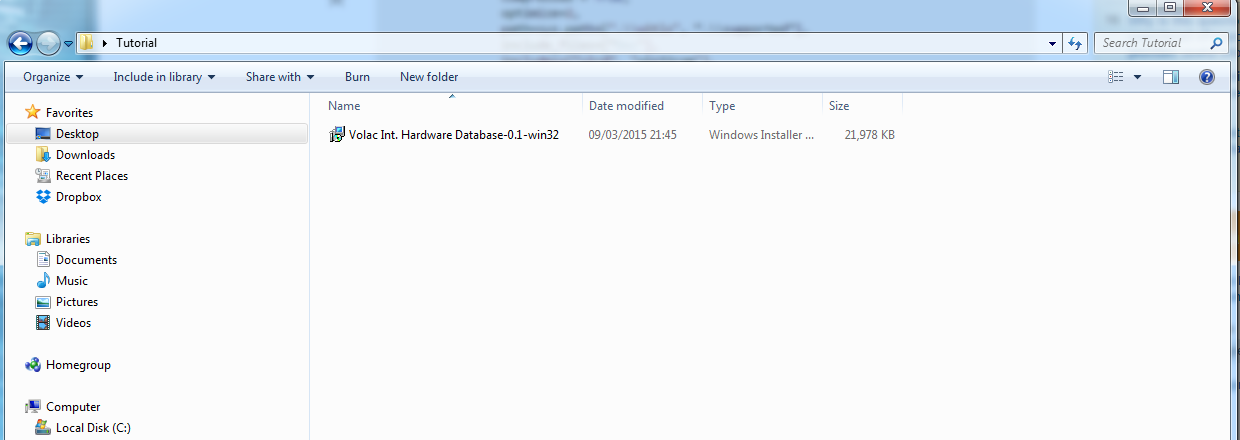
\includegraphics[width=\textwidth]{./Manual/Images/Tut1.png}
\end{figure}

\textbf{2) Double click the installer (left mouse button) and the setup will begin.}

\newpage

\textbf{3) The following window will appear, from here you may choose the location for the system to be installed to. By default it should install to "Program Files" for 32 bit computers or "Program File (x86)" for 64 bit computers.}

\begin{figure}[H]
    \includegraphics[width=\textwidth]{./Manual/Images/Tut2.png}
\end{figure}

\newpage

\textbf{4) Press the "Next" button to start the installation.}

\begin{figure}[H]
    \includegraphics[width=\textwidth]{./Manual/Images/Tut3.png}
\end{figure}

\newpage

\textbf{5) If the following warning message appears, press the "Yes" button to give permission for the installation to continue.}

\begin{figure}[H]
    \includegraphics[width=\textwidth]{./Manual/Images/Tut4.png}
\end{figure}

\newpage

\textbf{6) The installation should now begin. If the installer is no longer open, please see "step 2".}

\begin{figure}[H]
    \includegraphics[width=\textwidth]{./Manual/Images/Tut5.png}
\end{figure}

\newpage

\textbf{7) Press the "Finish" button after the installation has finished.}

\begin{figure}[H]
    \includegraphics[width=\textwidth]{./Manual/Images/Tut6.png}
\end{figure}

\newpage

\textbf{8) Navigate to the location the system was installed to and a folder called "Volac Int. Hardware Database" should be present.}

\begin{figure}[H]
    \includegraphics[width=\textwidth]{./Manual/Images/Tut7.png}
\end{figure}

\textbf{9) The program is now installed. The next section \ref{runprogram} will explain how to run your new system.}

\subsection{Running the System}\label{runprogram}

This section will be looking at how to run the system. If you have not yet installed the system onto your machine, please see the above section \ref{systeminstall}.

\newpage

\textbf{1) Locate the Windows Executable in the location where the system was installed.}

\begin{figure}[H]
    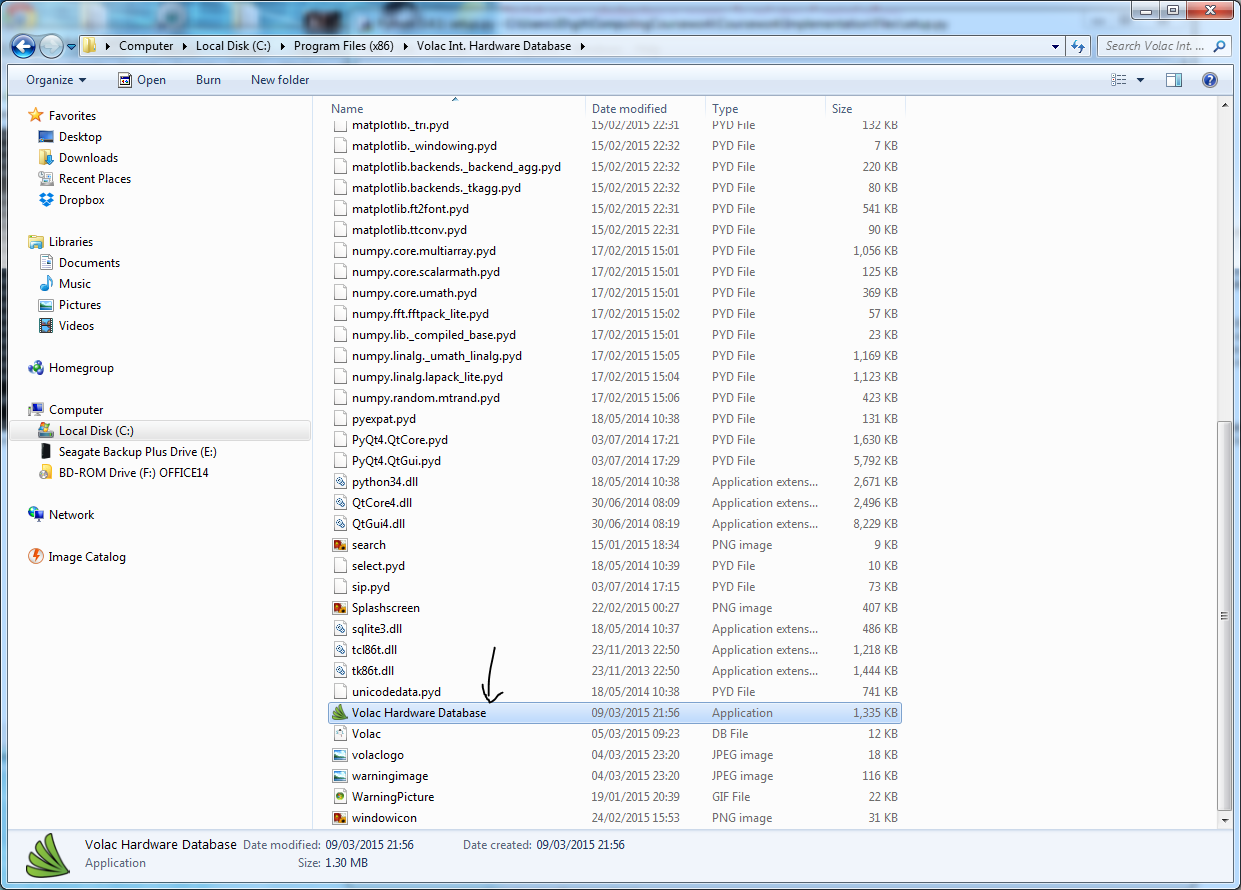
\includegraphics[width=\textwidth]{./Manual/Images/run1.png}
\end{figure}

\newpage

\textbf{Optional Step: 1.1) It is recommended that you create a shortcut so that it can be ran easier in the future. To do this "Right Click" the Executable and "Left Click" the "Create Shortcut" option.}

\begin{figure}[H]
    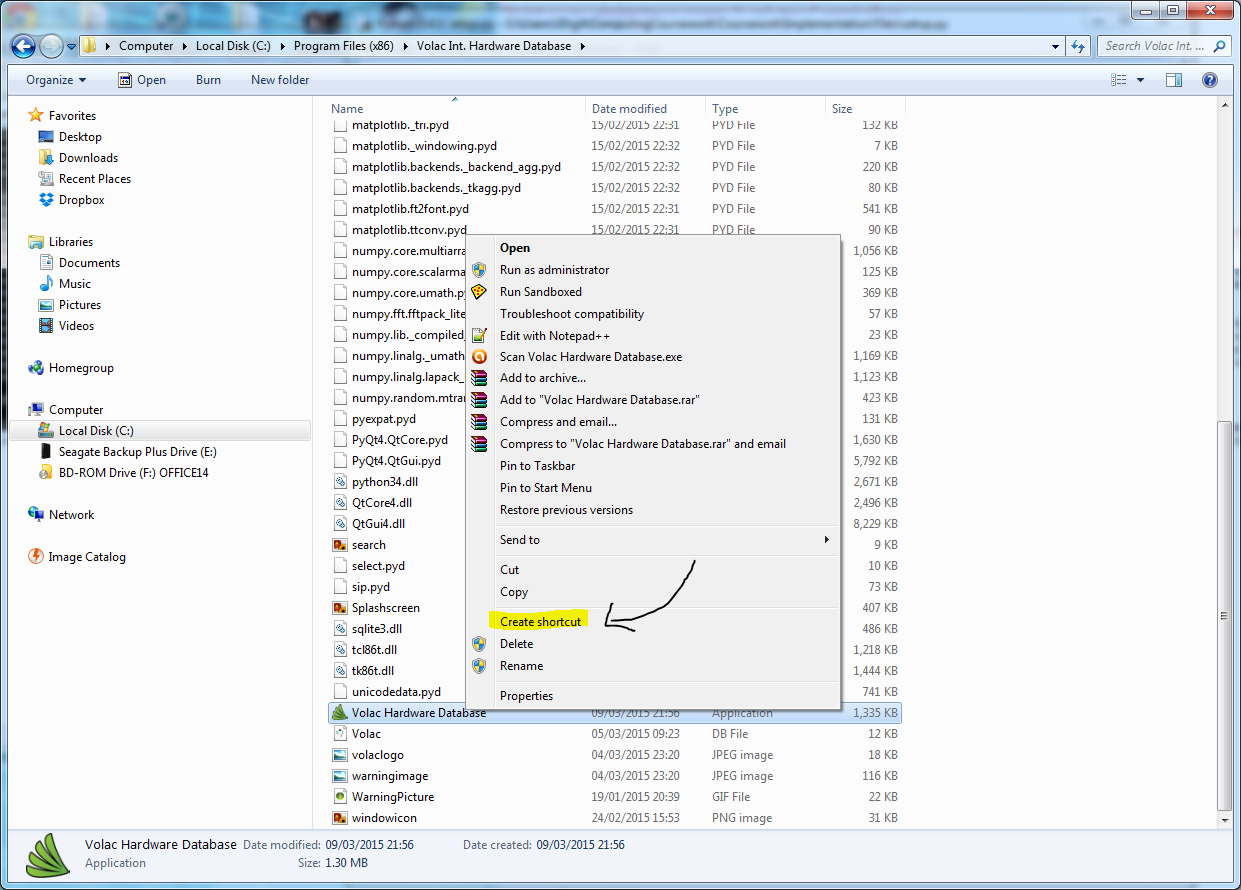
\includegraphics[width=\textwidth]{./Manual/Images/run2.png}
\end{figure}

\textbf{Optional Step: 1.2) The following warning message should appear. After clicking "Yes" a shortcut should be placed onto the Desktop.}

\begin{figure}[H]
    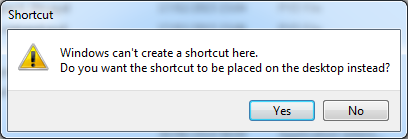
\includegraphics[width=\textwidth]{./Manual/Images/run3.png}
\end{figure}
\newpage

\textbf{Optional Step: 1.3) If the shortcut was created successfully an Executable should now be on your Desktop.}

\begin{figure}[H]
    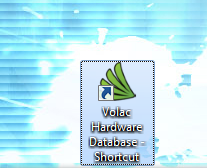
\includegraphics[width=\textwidth]{./Manual/Images/run4.png}
\end{figure}
\newpage

\textbf{2) Double click the Executable, either the original, or the shortcut if the above steps were followed.  If done correctly, the following screen should appear.}

\begin{figure}[H]
    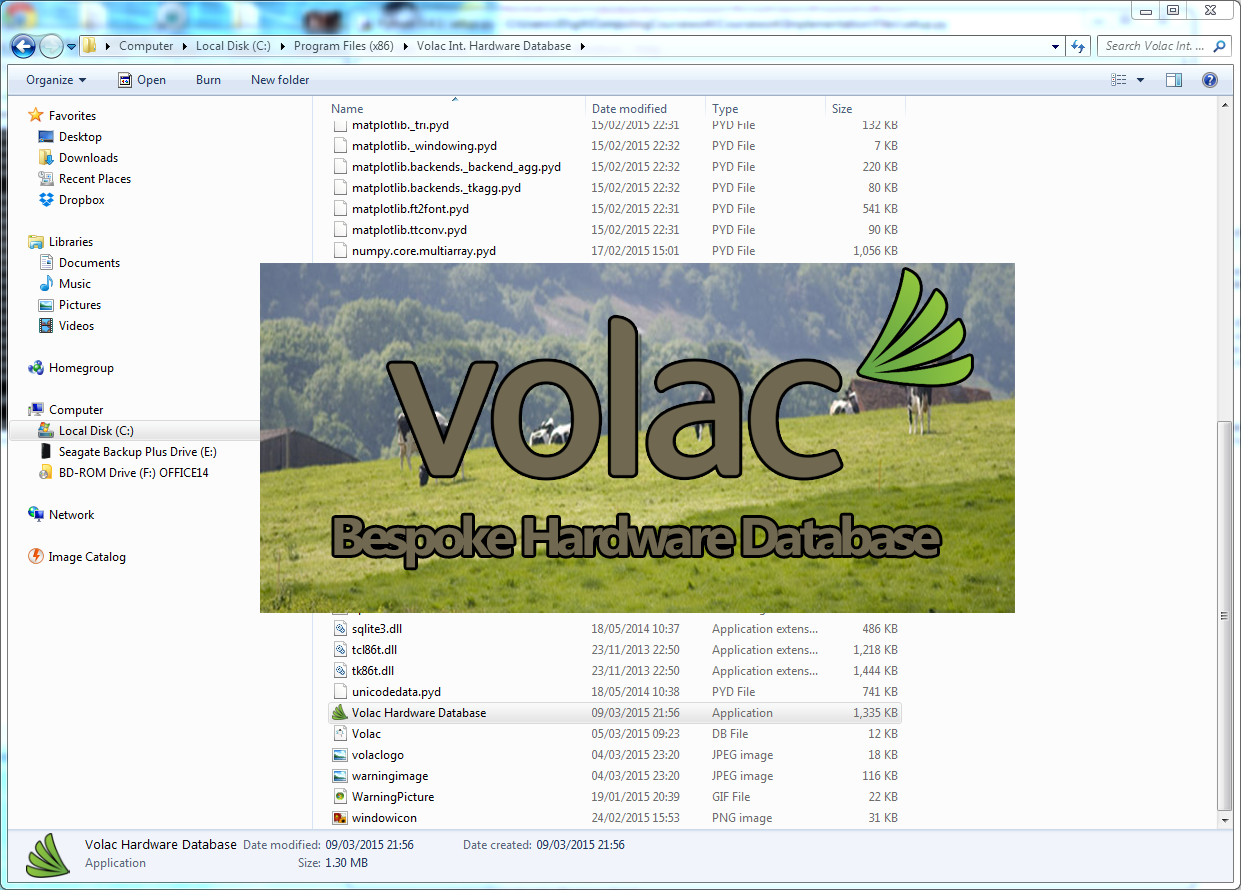
\includegraphics[width=\textwidth]{./Manual/Images/run5.png}
\end{figure}

\newpage

\textbf{3) After the program has loaded, the login screen should appear. The default Admin login will be: \newline
Username: "Admin" \newline
Password: "password"}

\begin{figure}[H]
    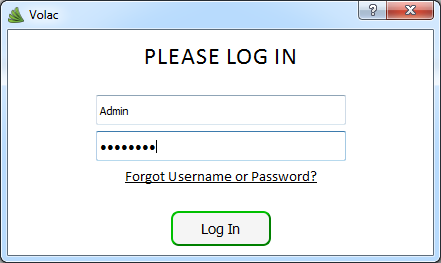
\includegraphics[width=\textwidth]{./Manual/Images/run6.png}
\end{figure}

\textbf{4) The program is now running and you should be able to gain access to the Admin Interface below.}

\begin{figure}[H]
    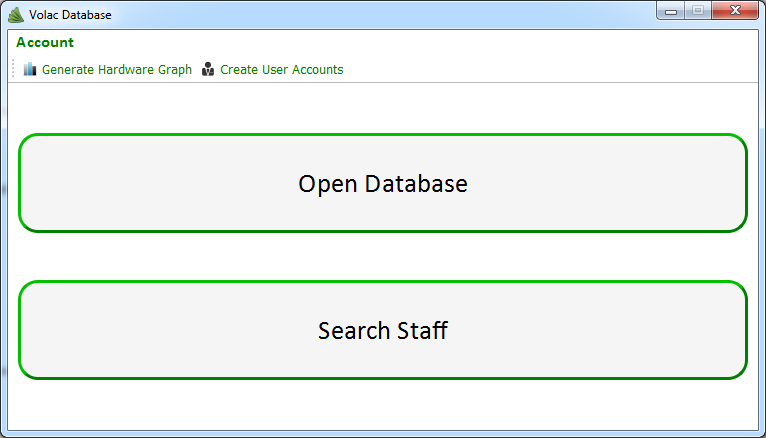
\includegraphics[width=\textwidth]{./Manual/Images/run7.png}
\end{figure}

\section{Tutorial}

\subsection{Introduction}

In this section I will be explaining how to use each part of the system. All tutorials have a step-by-step guide with annoted images to assist you in the best possible way.

\subsection{Assumptions}

I will assume that there is no prior knowledge of using computers since staff members at Volac International will have mixed levels of understanding to computer systems. To follow the tutorial the program must be already up and running, if it is not please follow the guide for "Running the System" \ref{runprogram}

\subsection{Tutorial Questions}

The following tutorials are split into a question and answer format.

%include as many subsubsections as necessary for each question in your list
General Tutorial

\subsubsection{How do I login to the system?}

To log in to the system you will first be required to have a user account. If you have data in the database then the IT Staff should have provided you with a login.

1) Open the system

2) Fill out your username and password

\begin{figure}[H]
    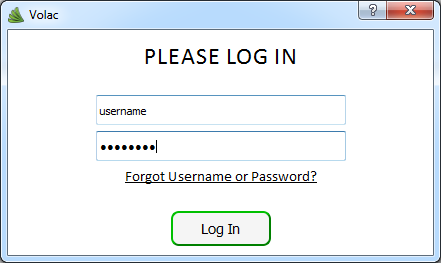
\includegraphics[width=\textwidth]{./Manual/Images/login1.png}
\end{figure}

3) Press Log In

\begin{figure}[H]
    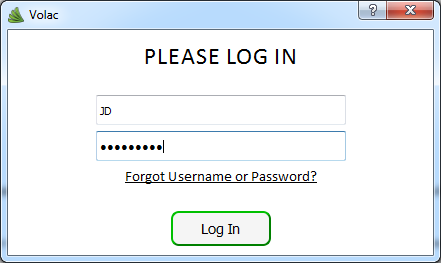
\includegraphics[width=\textwidth]{./Manual/Images/login2.png}
\end{figure}



If you have data but do not know your account. See section ----

Admin Interface Tutorial

\subsubsection{How do I open the database?}

\subsubsection{How do I view the different tables in the database?}

\subsubsection{How do I add data to the database?}

\subsubsection{How do I edit data in the database?}

\subsubsection{How do I delete data from the database?}

\subsubsection{How do I quick search for data in the database?}

\subsubsection{How do I generate a graph?}

\subsubsection{How do I add new accounts to the system?}

\subsubsection{How do I change my password?}

\subsubsection{How do I close the system?}

\subsubsection{How do I search for staff by department?}

Manager and Staff Interface Tutorial

\subsubsection{I forgot my password, how do I recover it?}

\subsubsection{How do I view staff in my department?}

\subsubsection{How do I view my own information?}

\subsubsection{How do I report a bug?}

\subsubsection{How do I report incorrect information?}

\subsubsection{How do I view my own information?}

\subsection{Saving}

\subsection{Limitations}

\section{Error Recovery}

%include as many subsections as necessary for each error
\subsection{Error 1}

\subsection{Error 2}

\section{System Recovery}

\subsection{Backing-up Data}

\subsection{Restoring Data}